\chapter{Framework: Pipes and Filters}

In this chapter, we design a framework based on the theoretical model from previous chapter. We start by establishing a small and general core architecture and continue with how we extended and used this core to build a flexible author-disambiguation tool. Implementation details of the framework and used algorithms and technologies in this framework will be discussed as well. Throughout the design, the requirements set in the foundation \autoref{foundation} and theoretical model were taken into account. At the end of the chapter we will discuss the strengts and weaknesses of the framework.

% aspect, flow, identifier, enrich, filter

\subsection{Small and Simple Core}

We opted for a small and simple core framework. It is based on Pipes and Filters with a few extension. We chose to use this design pattern for the following reasons:

\begin{enumerate}
\item \textbf{S
\end{enumerate}

\paragraph{Architecture}

\begin{figure}[htbp]
	\centering
		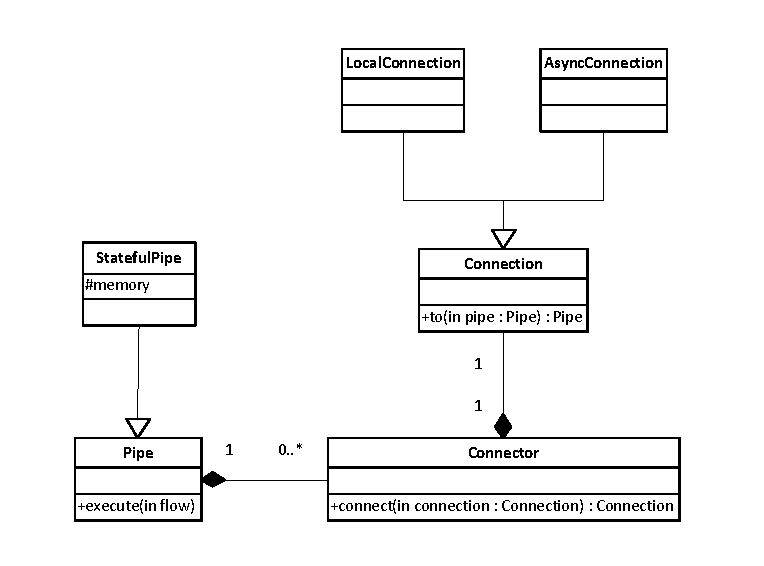
\includegraphics[width=0.65\textwidth]{fig/architecturev2}
	\caption{Pipes and Filters based Architecture.}
	\label{fig:architecturev2}
\end{figure}

\paragraph{Pipes and Connectors} +figuur

\paragraph{Connections} % niet beginnen over async stuff, later "gebruiken"

\subsection{Some useful pipes}

With these small and simple Pipes and Filters core we built some useful pipes along the way. Clearly the filter pipe is important to have in a Pipes and Filters architecture, so we explain this one first. Merging and Splitting flows, both extensively used pipes, are mentioned second. Last, we discuss two pipes more specific for our case but as yhey are used troughout the entire pipe system, we mention them here.

\paragraph{Filter} The Filter pipe allows us to filter flow in two ways, as you can also see on \autoref{fig:filter}. First, it is possible to test a condition for each arriving flow. Depending on this condition, the flow is forwarded to either the connector with identifier "true" or identifier "false". On top of that we are able to filter aspects of the flow itself. This Filter pipe gives us the possibility to control the flow in our pipe configuration. The flows should be small and contain only aspects that are necessary.

\begin{figure}[htbp]
	\centering
		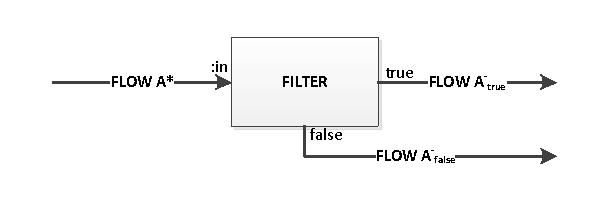
\includegraphics[width=0.65\textwidth]{fig/filter}
	\caption{Filter pipe.}
	\label{fig:filter}
\end{figure}

\paragraph{Merge and Split} In the case we want to forward the result from one pipe to multiple pipes or from multiple pipes to one, we need a Split or Merge pipe. Split pipes have the default ":in" connector and split their input over $n$ output connectors identified by $1,\ldots,n$. A Merge pipe does the inverse by merging input connections $1,\ldots,n$ into one connector identified by the default ":out".

\begin{figure}[htbp]
	\centering
		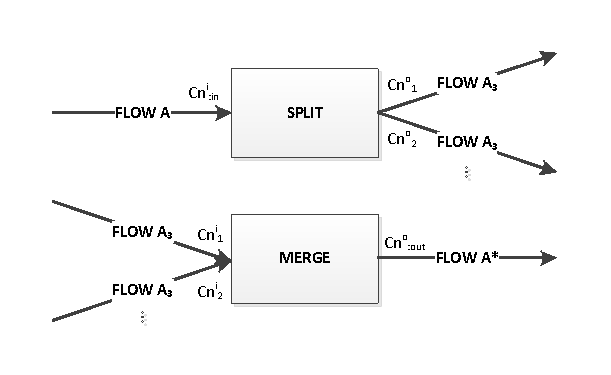
\includegraphics[width=0.65\textwidth]{fig/mergeandsplit}
	\caption{Merge and Split pipes.}
	\label{fig:mergeandsplit}
\end{figure}

\paragraph{Persist Discovery}

\paragraph{Persist Fact}

\subsection{Extending to fit our needs}

\paragraph{Pipes with memory} 

\paragraph{Flow enrichment}

\paragraph{Parsers}

\paragraph{Asynchronous connections}

\paragraph{Locking}

\section{Practical applications}

\subsection{Dependency Resolution}

\subsection{Concurrent, incremental Clustering}

Clustering is a very important step in building towards a solution. Each new flow of information indirectly leads to a clustering operation. Acquiring new information triggers rules which on their turn yield similarities. These similarities change the balance between clusters. In the worst case, an expensive rebalancing procedure is necessary.

It is obvious that processing similarities is something that will be executed very frequently (numbers?). The combination of the enormous amount of similarities and their expensive processing requires us to make this process as streamlined and efficient as possible. The clustering algorithm as explained in [REF] leads to a first, na\"ive implementation approach. Rethinking the absolute needs of the clustering algorithm then leads to a second approach that benifits greatly of the foundations of our framework.

\paragraph{In-graph implementation} The most simple solution one can think of is to maintain the ICW and OCW for every vertex in the vertex itself. The adjacency matrix would implicitly be defined by the edges between two nodes in the similarity plane. This technique has two main drawbacks:

\begin{enumerate}
\item A lot of load would be pushed to the database.
\item There would be a need for several concurrency control mechanisms/
\end{enumerate}

If clustering could be executed without the use of the database in an efficient manner, it would be preferrable. After all it is in our best interest to take as much load as possible away from the database because it is much more difficult to scale than our pipes and filters architecture. Besides, the similarity ``meta''-plane is not something that should be queried from our end-user application. The users are interested in the result of the clustering, not the way it got there.

In the case of similarities being processed in parallel, we need to pay some extra attention. We do not want that the clustering mechanism inflicts race conditions and, by consequence, inconsistencies on the graph.


\paragraph{As a stateful pipe}

\begin{algorithm}
\caption{!!!}
\label{mincutgusfield}
\begin{algorithmic}
\STATE \textbf{lock} $I_1,I_2$
\IF{cluster($I_1$) == cluster($I_2$)}
  \STATE \textbf{watch} $C_1,C_2$
  \STATE \textbf{unlock} $I_1,I_2$
  \STATE \textbf{process(intra-cluster)}
\ELSE
  \STATE \textbf{lock} $C_1,C_2$
  \STATE \textbf{unlock} $I_1,I_2$
  \STATE \textbf{process(inter-cluster)}
  \STATE \textbf{execute}
  \STATE \textbf{unlock} $C_1,C_2$
\ENDIF
\end{algorithmic}
\end{algorithm}

\begin{figure}[htbp]
	\centering
		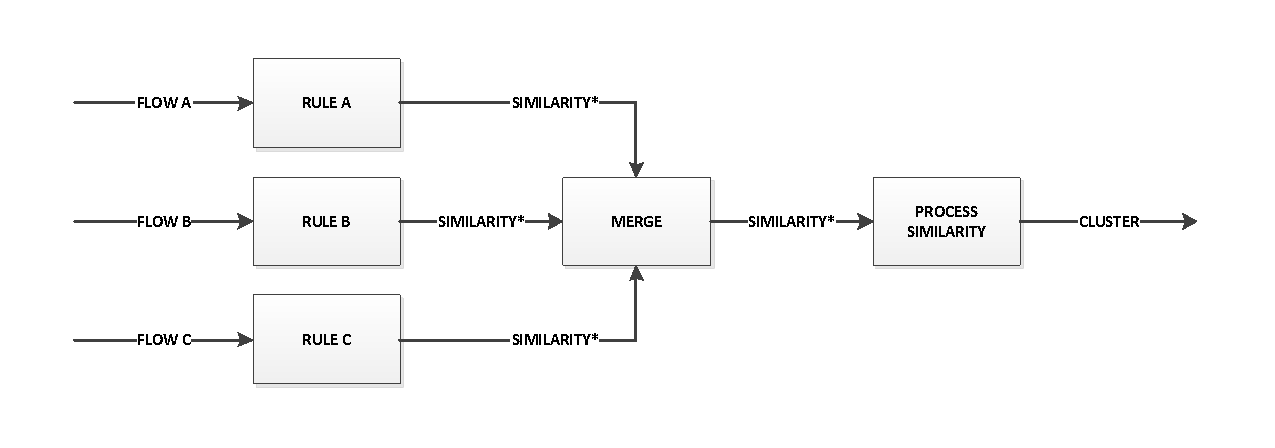
\includegraphics[width=1\textwidth]{fig/clusteringpipe}
	\caption{Clustering flow}
	\label{fig:clusteringpipe}
\end{figure}

\subsection{Assignment of e-mail addresses}